\documentclass{standalone}

\usepackage{hyperref}
\usepackage{graphicx}
\usepackage{amsmath}
\usepackage{amssymb}
\usepackage{lmodern}
\usepackage{tikz}
\usetikzlibrary{shapes.geometric,shapes.arrows,decorations.pathmorphing,decorations.markings}
\usetikzlibrary{matrix,chains,scopes,positioning,arrows,fit,spy}
\usepackage{pgfplots}
\pgfplotsset{width=10cm,compat=1.9}
\usepgfplotslibrary{external}

\begin{document}

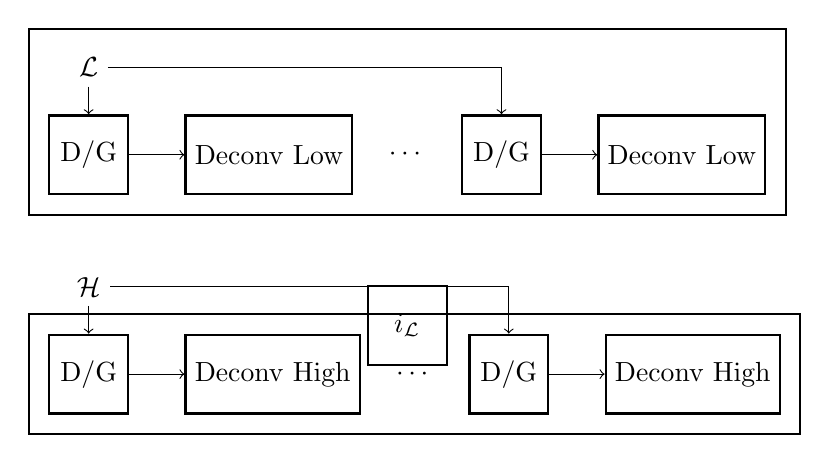
\begin{tikzpicture}
\node (low_mc1_dg) at (0,0) [draw, thick, minimum size=1cm] {D/G};
\node (low_mc1_deconv) at (low_mc1_dg.east) [draw, thick, minimum width=1cm, minimum height=1cm, right=20pt] {Deconv Low};
\node (low_ell) at (low_mc1_deconv.east) [minimum width=1cm, minimum height=1cm, right=5pt] {$\cdots$};
\node (low_mcn_dg) at (low_ell.east) [draw, thick, minimum width=1cm, minimum height=1cm, right=5pt] {D/G};
\node (low_mcn_deconv) at (low_mcn_dg.east) [draw, thick, minimum width=1cm, minimum height=1cm, right=20pt] {Deconv Low};
\node (low_vis) at (low_mc1_dg.north)[above=10pt]{$\mathcal{L}$};

\draw [->] (low_mc1_dg) edge (low_mc1_deconv); 
\draw [->] (low_mcn_dg) edge (low_mcn_deconv);
\draw [->] (low_vis) edge (low_mc1_dg);
\draw [->, to path={-| (\tikztotarget)}] (low_vis) edge (low_mcn_dg);

\node[fit=(low_mc1_dg)(low_mc1_deconv)(low_mcn_dg)(low_mcn_deconv)(low_vis), draw, thick, inner sep=7pt](lowres_step){};

\node (lowres_recon) at (lowres_step.south) [draw, thick, minimum size=1cm, below=25pt] {$i_\mathcal{L}$};

\node (full_mc1_dg) at (low_mc1_dg.south) [draw, thick, minimum size=1cm, below=50pt] {D/G};
\node (full_mc1_deconv) at (full_mc1_dg.east) [draw, thick, minimum width=1cm, minimum height=1cm, right=20pt] {Deconv High};
\node (full_ell) at (full_mc1_deconv.east) [minimum width=1cm, minimum height=1cm, right=5pt] {$\cdots$};
\node (full_mcn_dg) at (full_ell.east) [draw, thick, minimum width=1cm, minimum height=1cm, right=5pt] {D/G};
\node (full_mcn_deconv) at (full_mcn_dg.east) [draw, thick, minimum width=1cm, minimum height=1cm, right=20pt] {Deconv High};
\node (full_vis) at (full_mc1_dg.north)[above=10pt]{$\mathcal{H}$};

\draw [->] (full_mc1_dg) edge (full_mc1_deconv); 
\draw [->] (full_mcn_dg) edge (full_mcn_deconv);
\draw [->] (full_vis) edge (full_mc1_dg);
\draw [->, to path={-| (\tikztotarget)}] (full_vis) edge (full_mcn_dg);

\node[fit=(full_mc1_dg)(full_mc1_deconv)(full_mcn_dg)(full_mcn_deconv), draw, thick, inner sep=7pt](fullres_step){};

\end{tikzpicture}

\end{document}